
\section{Implémentation}
Pour tester les algorithmes de mesure avec des vidéos sur le terrain,
Dr. Mudry Pierre-André et M. Matter Fabien nous on aimablement laissé accès à
la caméra de notre projet parent \emph{VibroSnow\cite{VibroSnow}} et nous
les remercions énormément.

\subsection{Récupération des vidéos}
La caméra de \emph{VibroSnow} détecte le passage d'objet (voitures, chute de neige,...) et
enregistre une vidéo qui est ensuite transmise à un serveur \emph{Windows}.
Bien que l'accès aux vidéos nous a été donné, nous ne pouvons pas aller chercher les vidéos
directement sur le serveur \emph{Windows} car il est utilisé pour d'autres projets auxquels nous
n'avons pas accès.\\
Il a donc fallu créer un script \emph{Powershell}, transferant chaque jour les vidéos
cumulées sur le serveur \emph{Windows} vers un serveur auquel nous avons accès.
Un \emph{Raspberry Pi} a été mis en place comme serveur pour récuperer les vidéos.

\subsection{Mesure du débit de chute de neige}
La méthode utilisée pour détecter les chutes de neige se décompose ainsi :
\begin{description}
    \item[Soustraction de deux images] \hfill \\
    pour isoler les éléments qui ont bougé entre les deux images
    \item[Seuillage des niveaux de blancs sur l'image] \hfill \\
    pour accentuer les chutes de neige
    \item[Calcul du ratio de pixels blancs] \hfill \\
    pour avoir un nombre correspondant au débit de chute de neige    
\end{description}

\begin{figure}[H]
    \begin{subfigure}{.45\textwidth}
        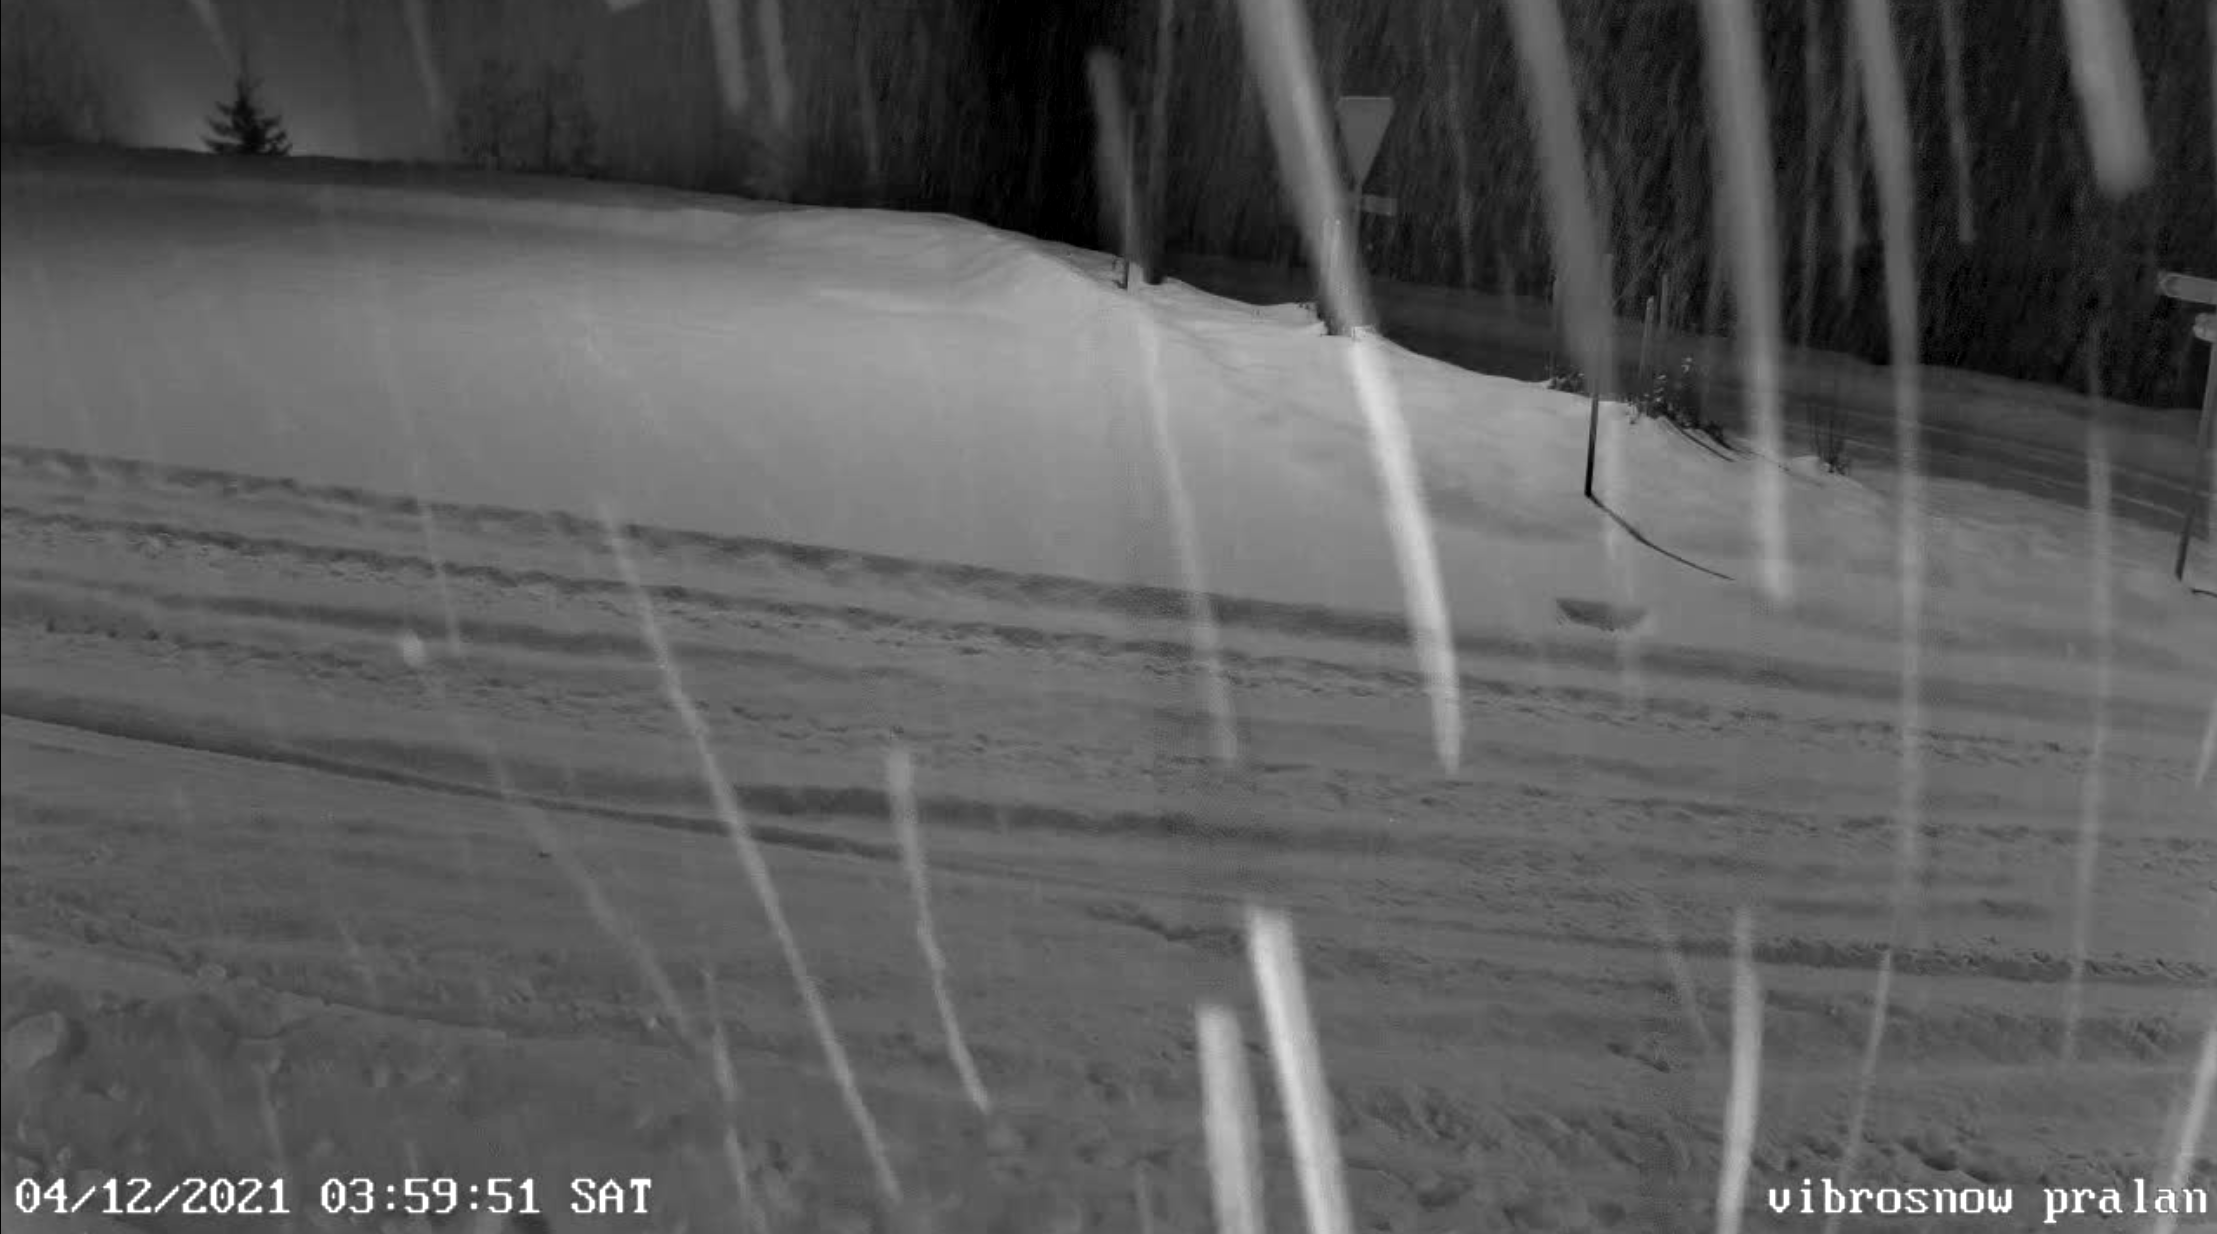
\includegraphics[width=\linewidth]{Images/computer_vision/snowfall/original.png}
        \caption{Image originale}
        \label{fig:Snowfall_original}
    \end{subfigure}
    \hfill
    \begin{subfigure}{.45\textwidth}
        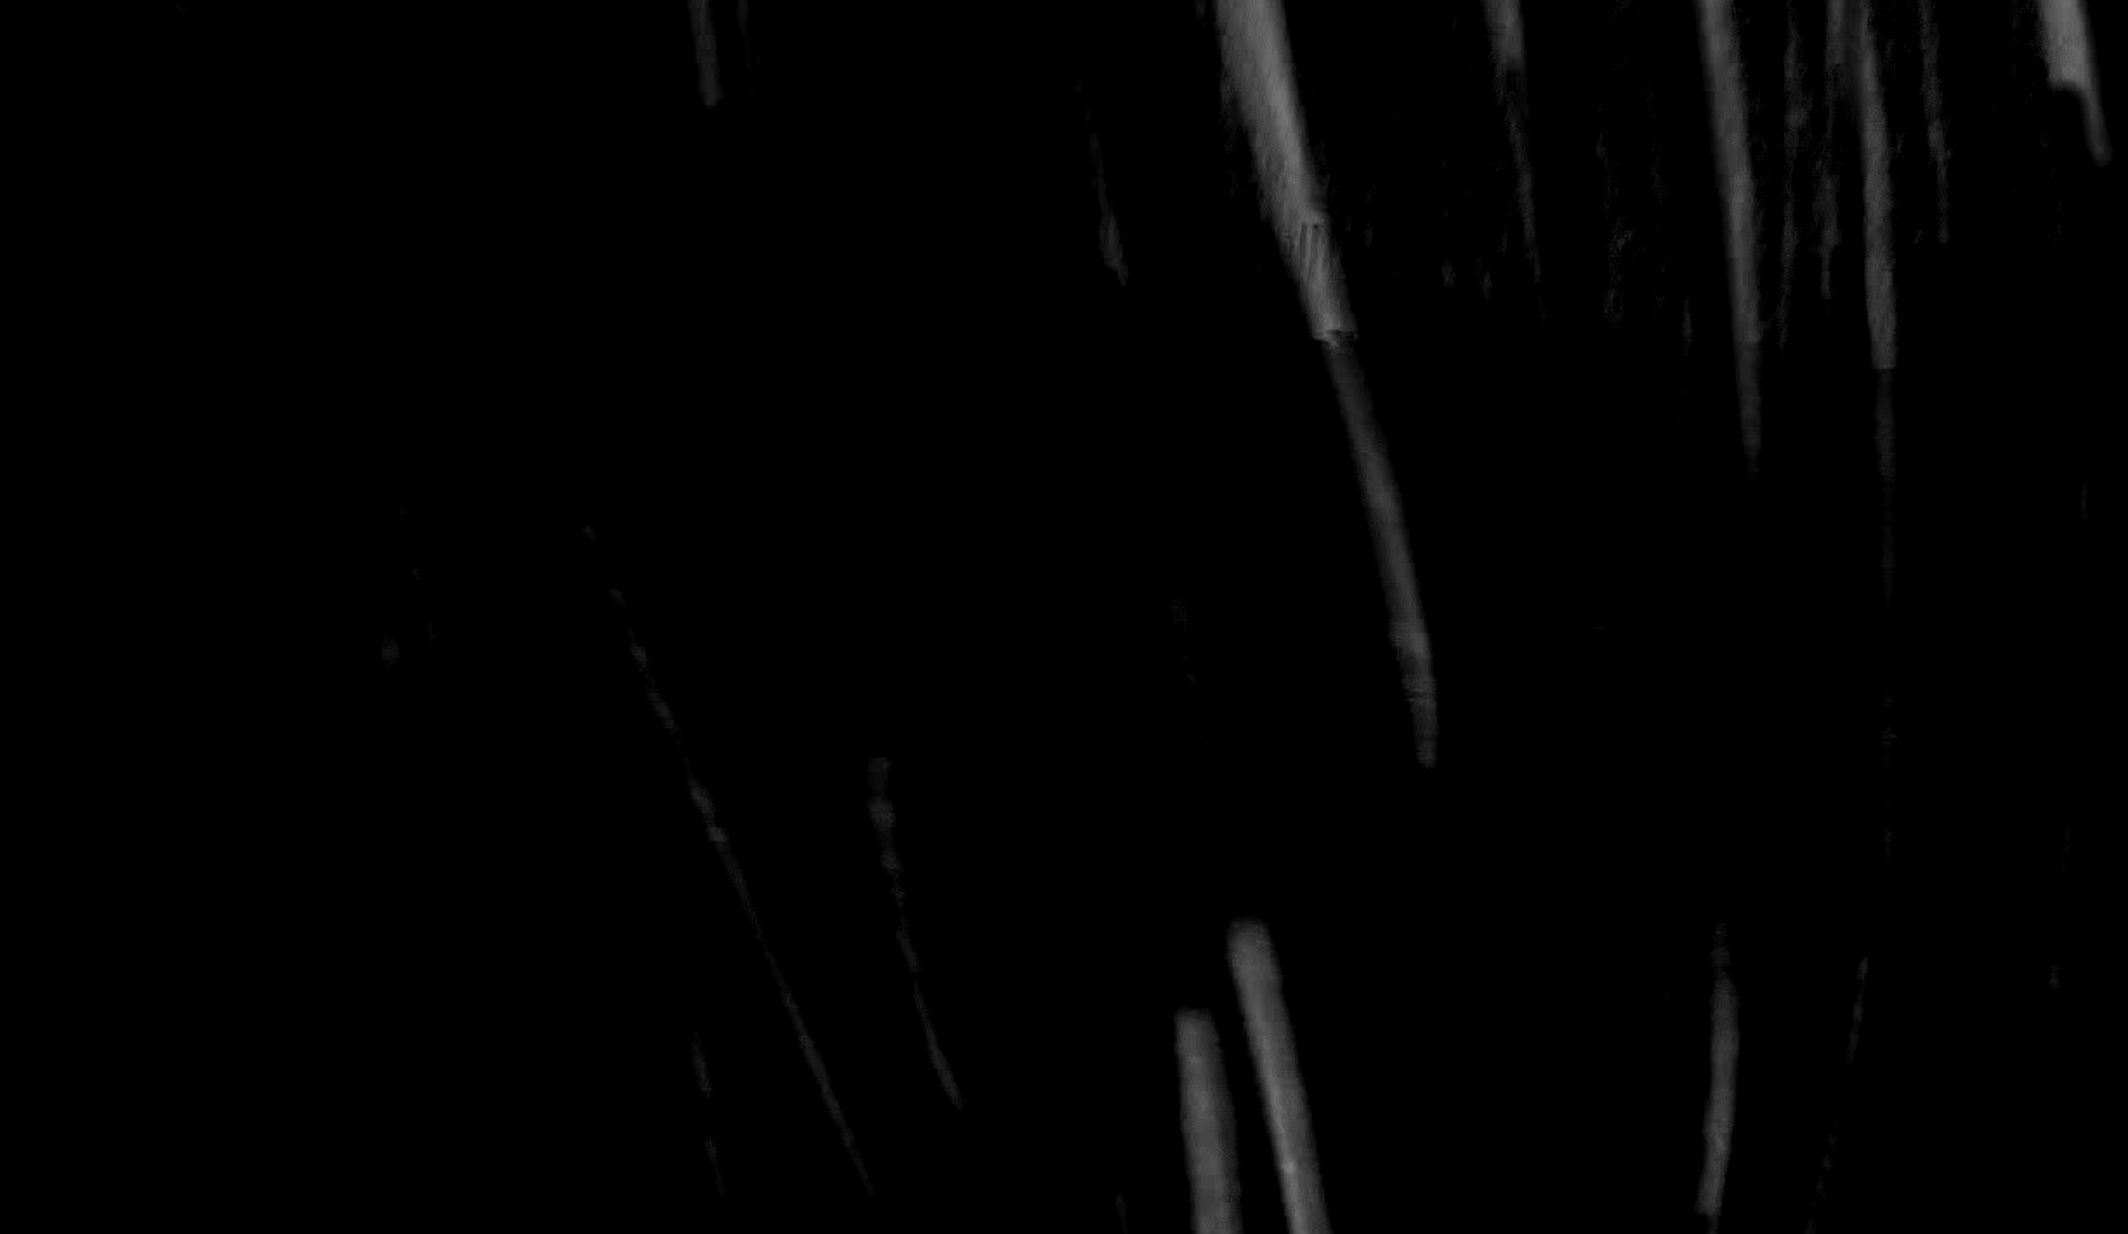
\includegraphics[width=\linewidth]{Images/computer_vision/snowfall/noise.png}
        \caption{Image avec neige isolée}
        \label{fig:Snowfall_noise}
    \end{subfigure}
    \hfill
    \centering
    \begin{subfigure}{.45\textwidth}
        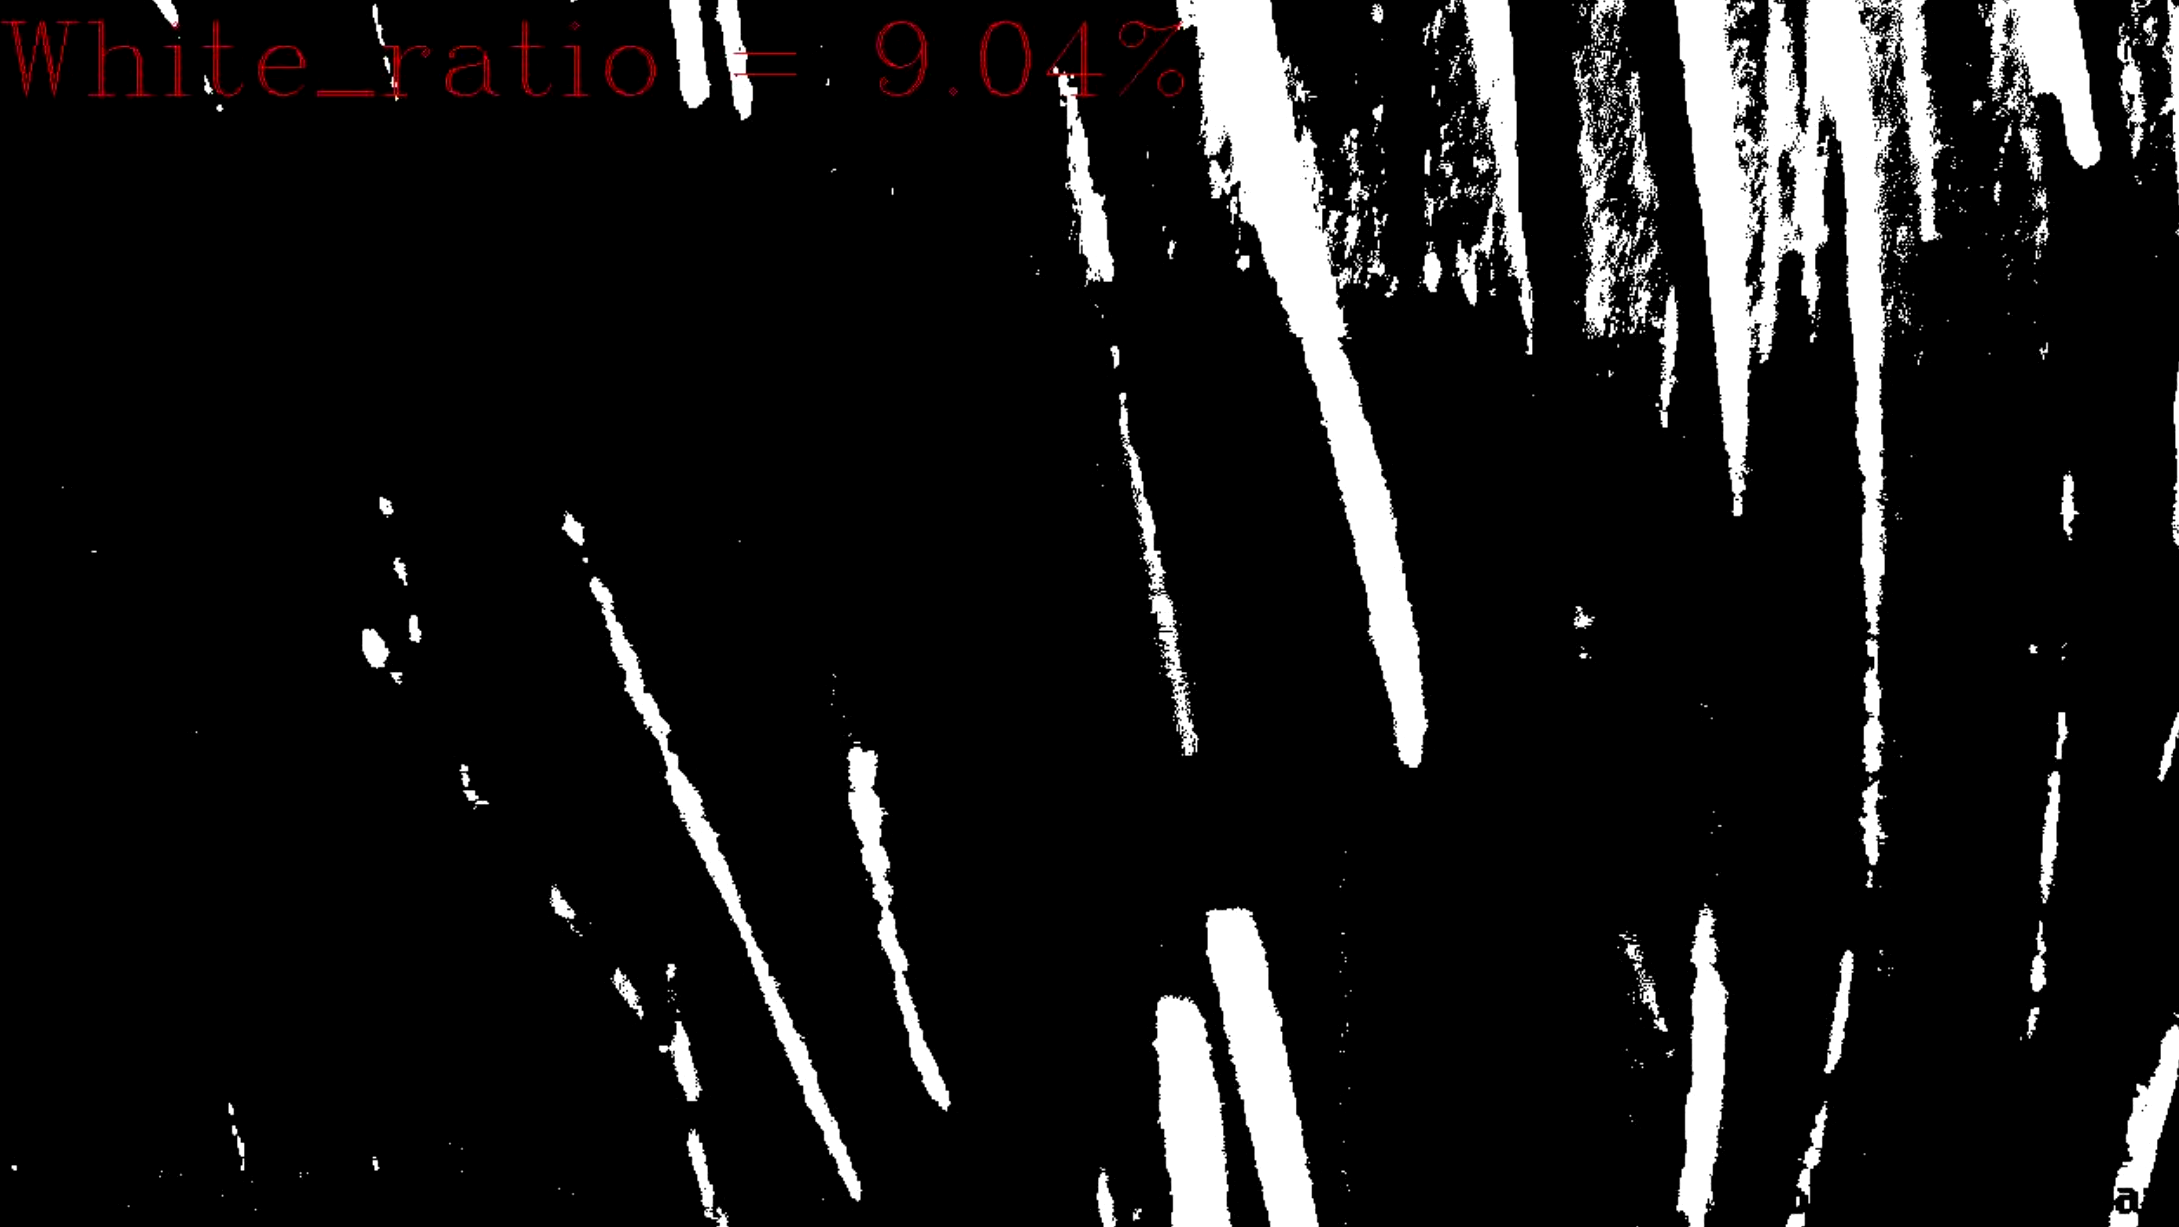
\includegraphics[width=\linewidth]{Images/computer_vision/snowfall/snowfall.png}
        \caption{Image seuillée avec calcul du ratio de pixels blancs (9.05\% ici)}
        \label{fig:Snowfall_thres}
    \end{subfigure}
    \caption{Étapes de la mesure de débit de chute de neige}
    \label{fig:Snowfall_algorithm}
\end{figure}
\newpage

\subsection{Détection de route enneigée} \label{snowOnRoad}
Deux méthodes ont été testées pour détecter si la route est enneigée ou non.\\
La première réalise un simple seuillage des niveaux de blancs, et un calcul
du ratio des pixels blancs sur l'image. On récupère plusieurs images et on
calcul la moyenne du ratio de blanc sur toute les images.
Cette moyenne est ensuite comparée à une moyenne similaire réalisée sur une
vidéo de la route déneigée, en vérifiant qu'on se trouve au même moment de
la journée (jour/nuit, matin/après-midi).\\
La deuxième est identique, à l'exception d'une suppression du bruit réalisée
avant le seuillage. Cette suppresion du bruit reprends la méthode d'isolation
de neige utilisée pour mesurer le débit de chute de neige et soustrait cette image
de bruit à l'image originale. Cette méthode demande un peu plus de calculs mais peut
potentiellement générer un résultat plus fiable.

\begin{figure}[H]
    \begin{subfigure}{.45\textwidth}
        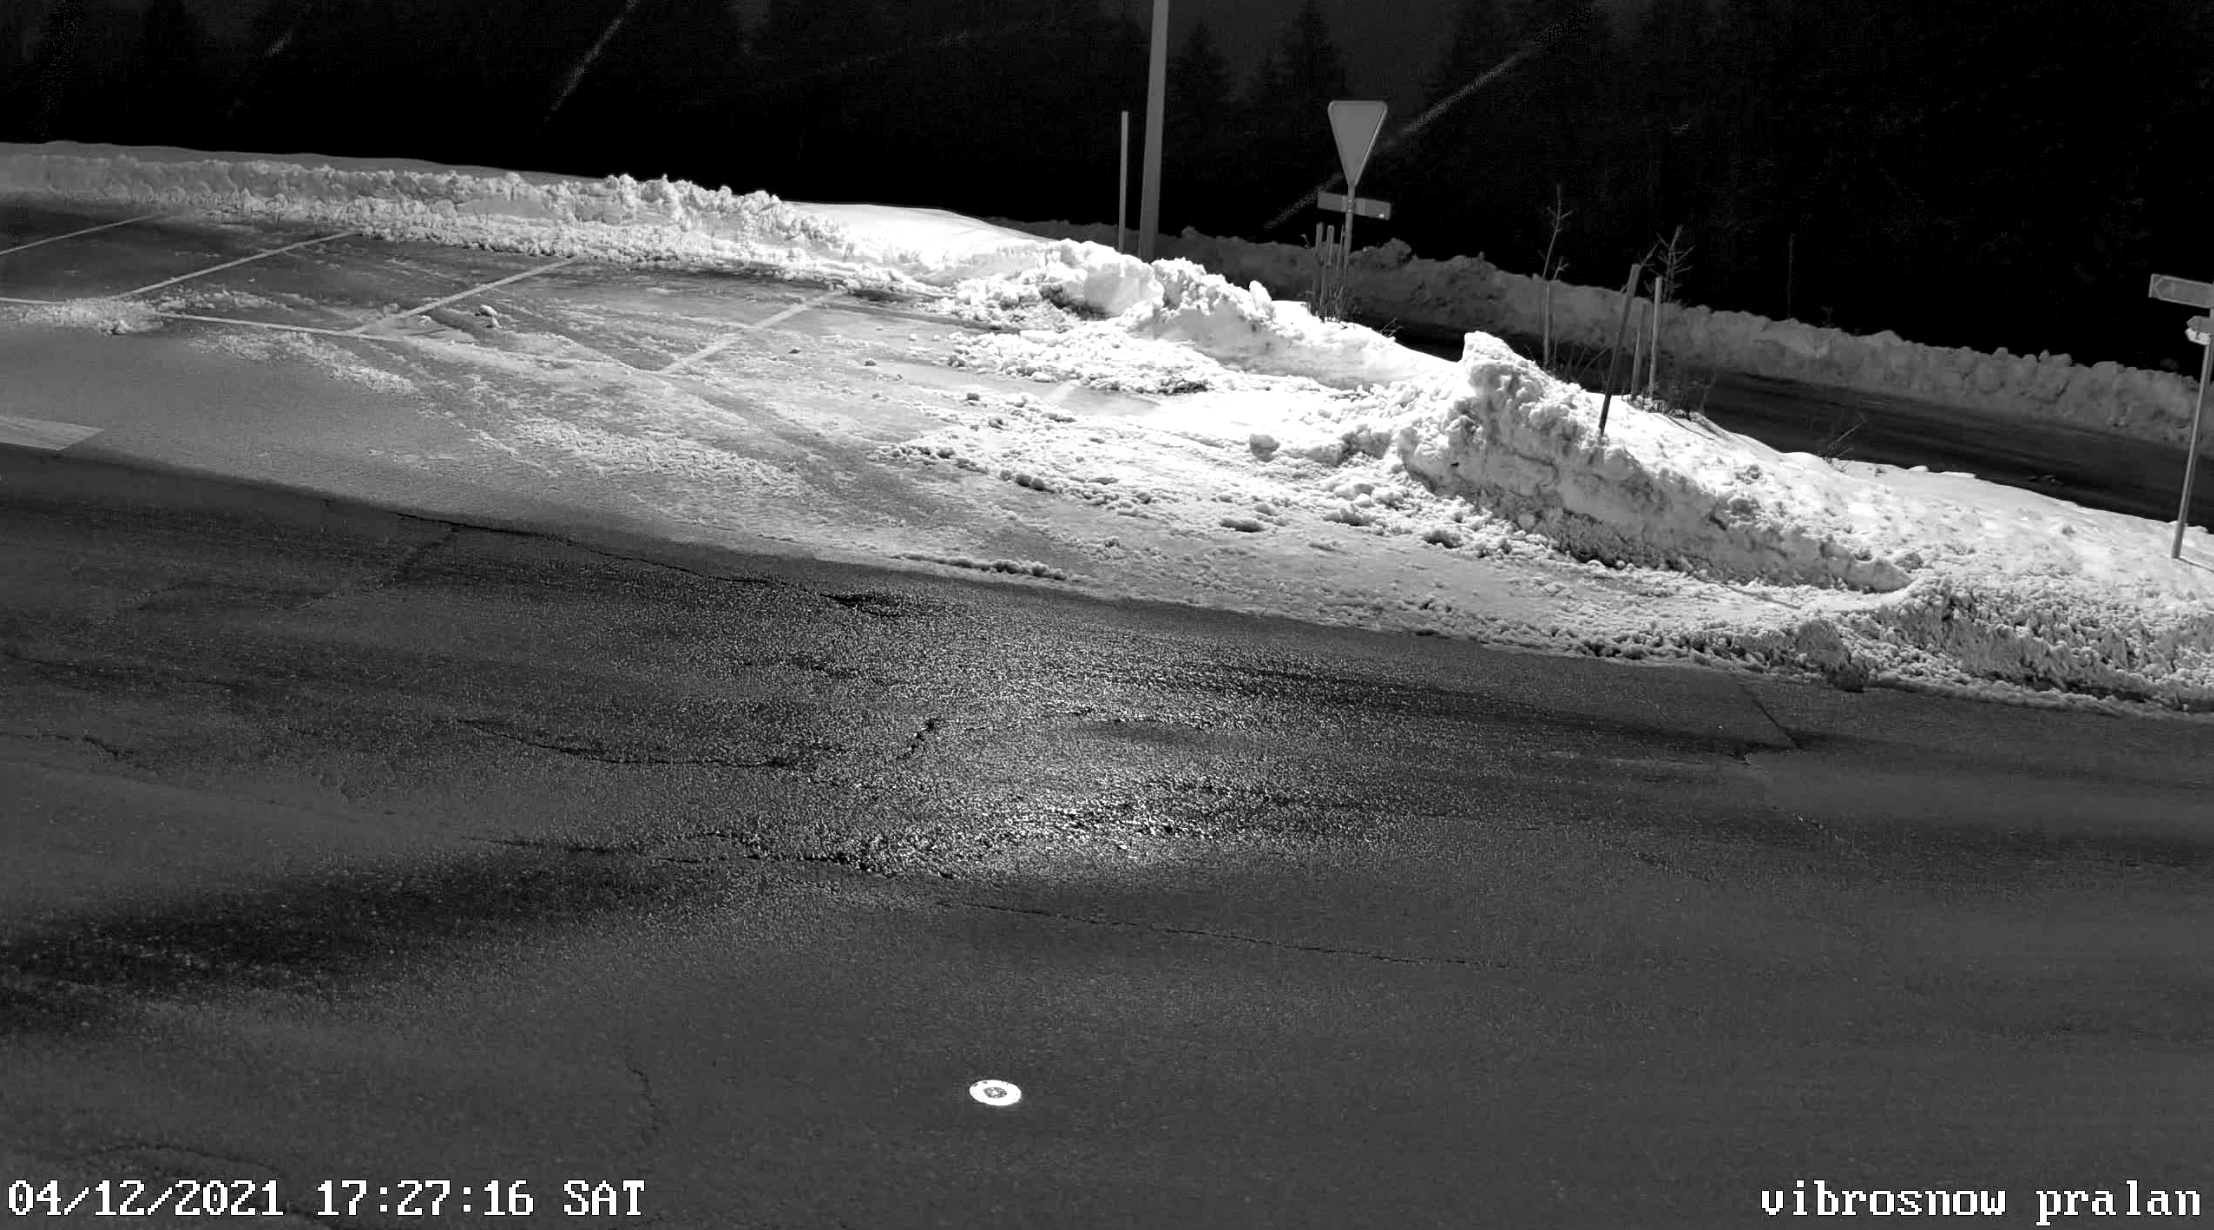
\includegraphics[width=\linewidth]{Images/computer_vision/snowOnRoad/ref_original.png}
        \caption{Image de référence originale}
        \label{fig:SnowOnRoad_ref_original}
    \end{subfigure}
    \hfill
    \begin{subfigure}{.45\textwidth}
        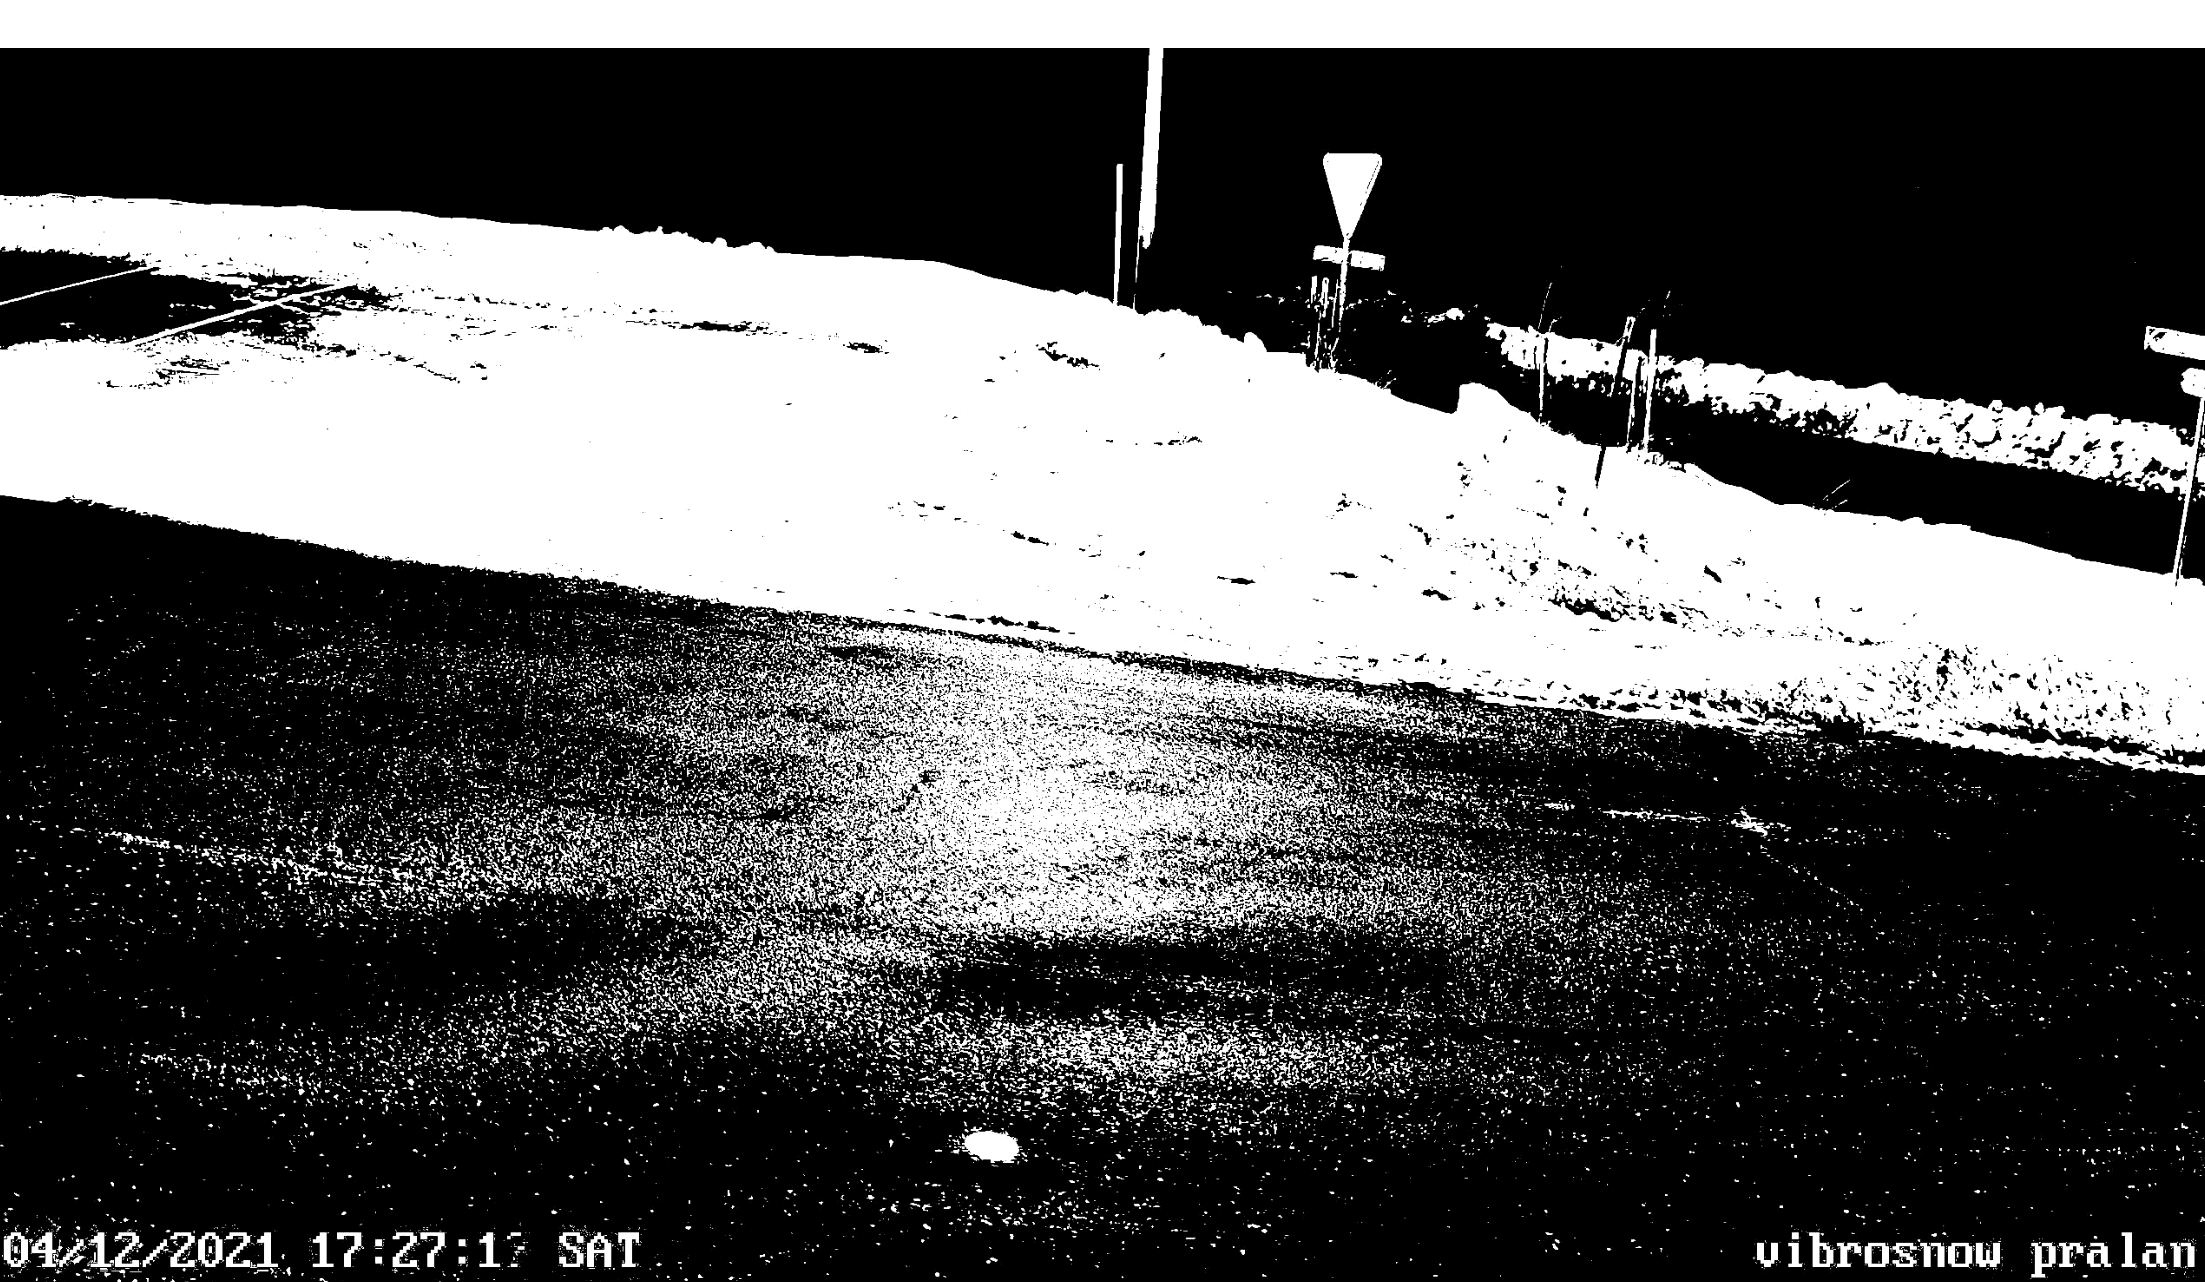
\includegraphics[width=\linewidth]{Images/computer_vision/snowOnRoad/ref_thres.png}
        \caption{Image de référence seuillée}
        \label{fig:SnowOnRoad_ref_thres}
    \end{subfigure}
    \caption[Référence pour détection de neige sur route]{Image de référence}
    \label{fig:SnowOnRoad_ref}
\end{figure}

\begin{figure}[H]
    \begin{subfigure}{.45\textwidth}
        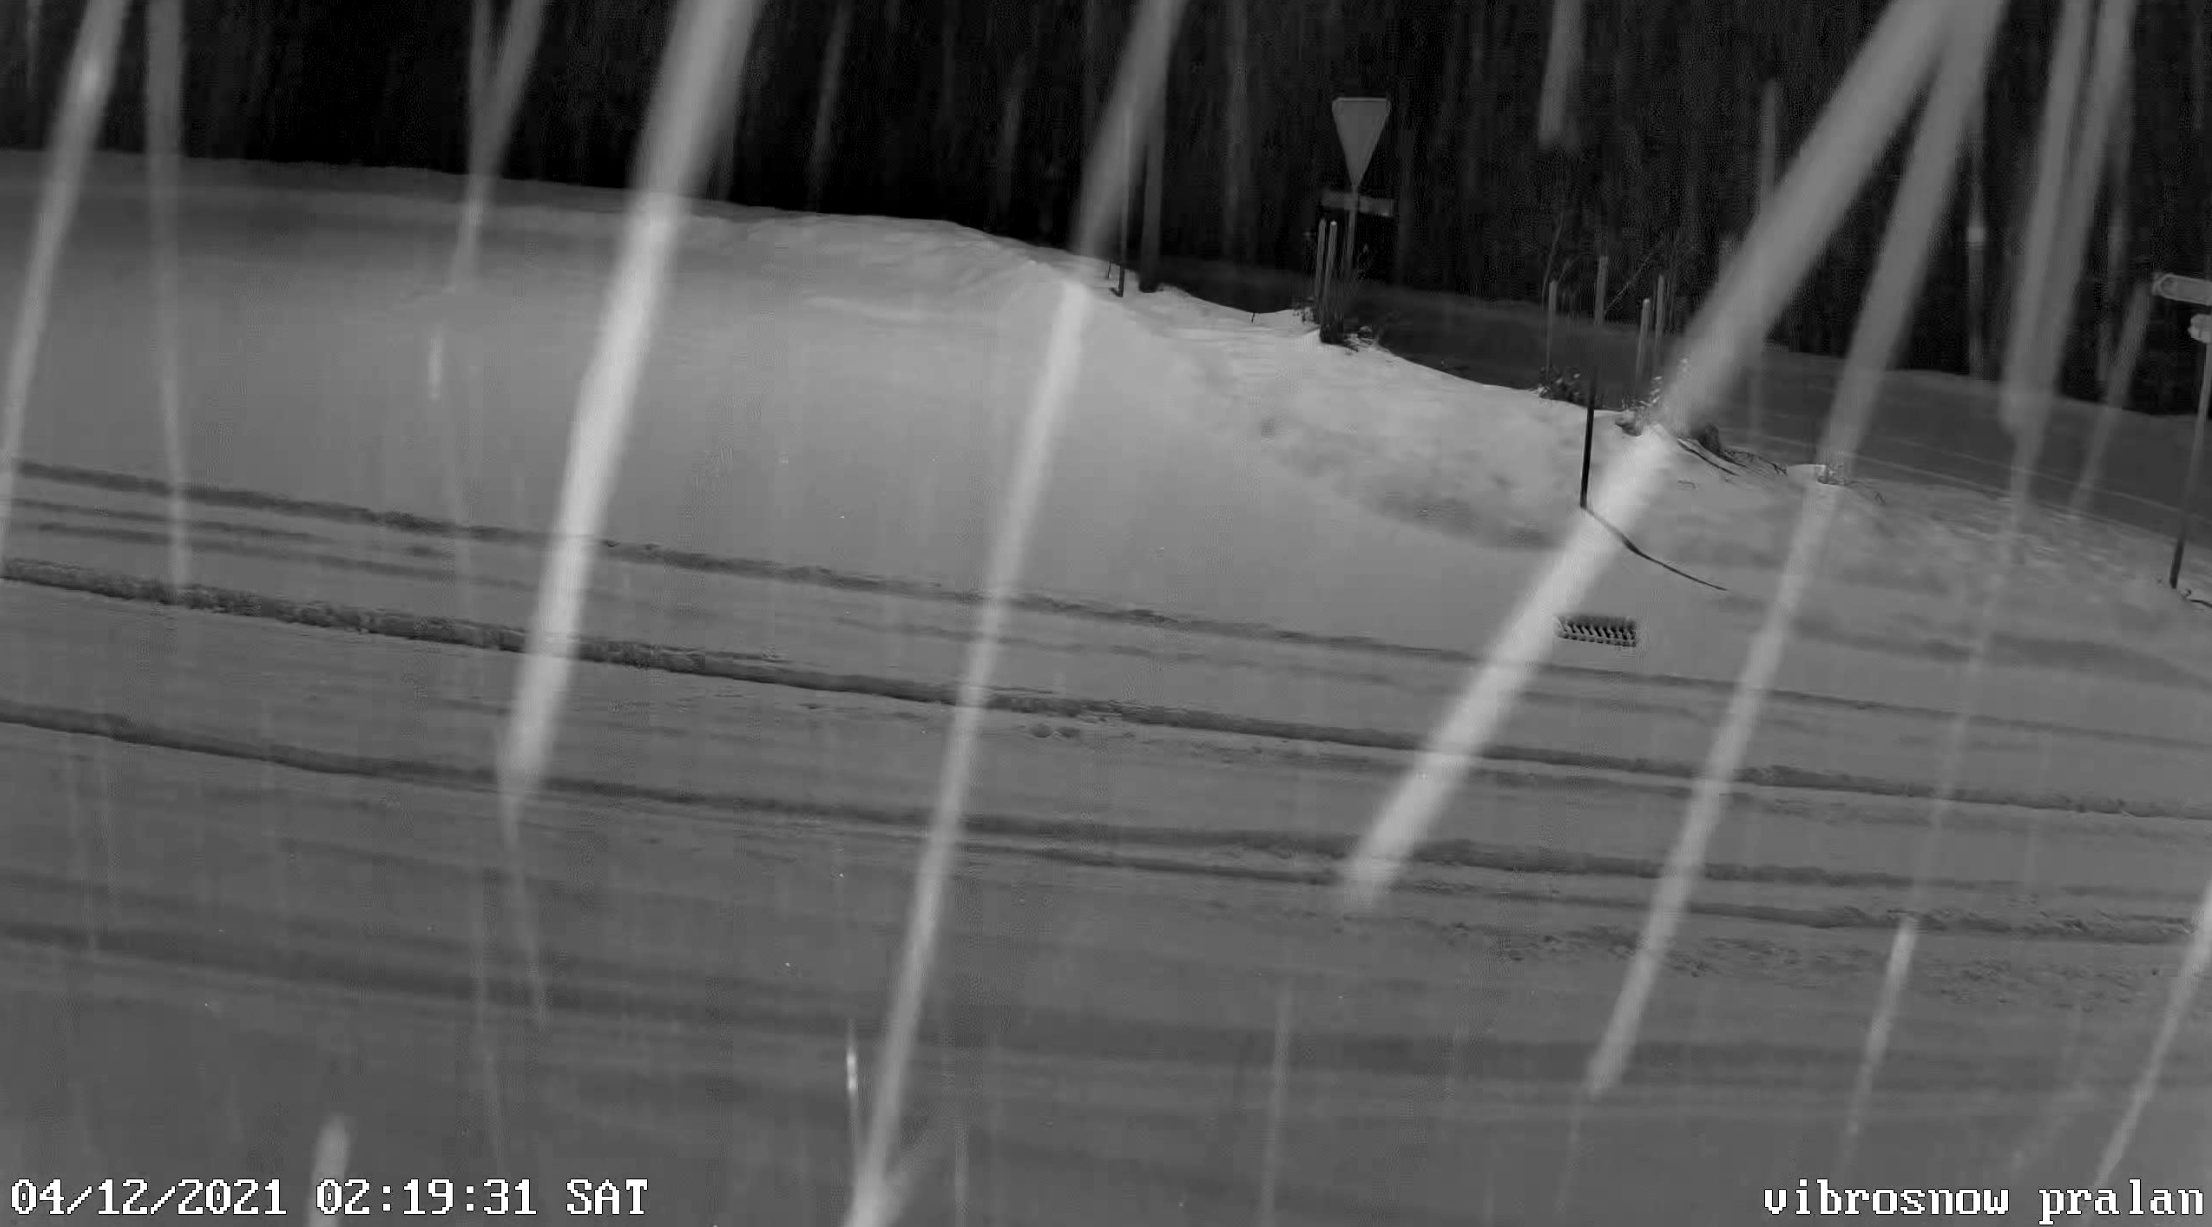
\includegraphics[width=\linewidth]{Images/computer_vision/snowOnRoad/test_original.png}
        \caption{Image de test originale}
        \label{fig:SnowOnRoad_test_original}
    \end{subfigure}
    \hfill
    \begin{subfigure}{.45\textwidth}
        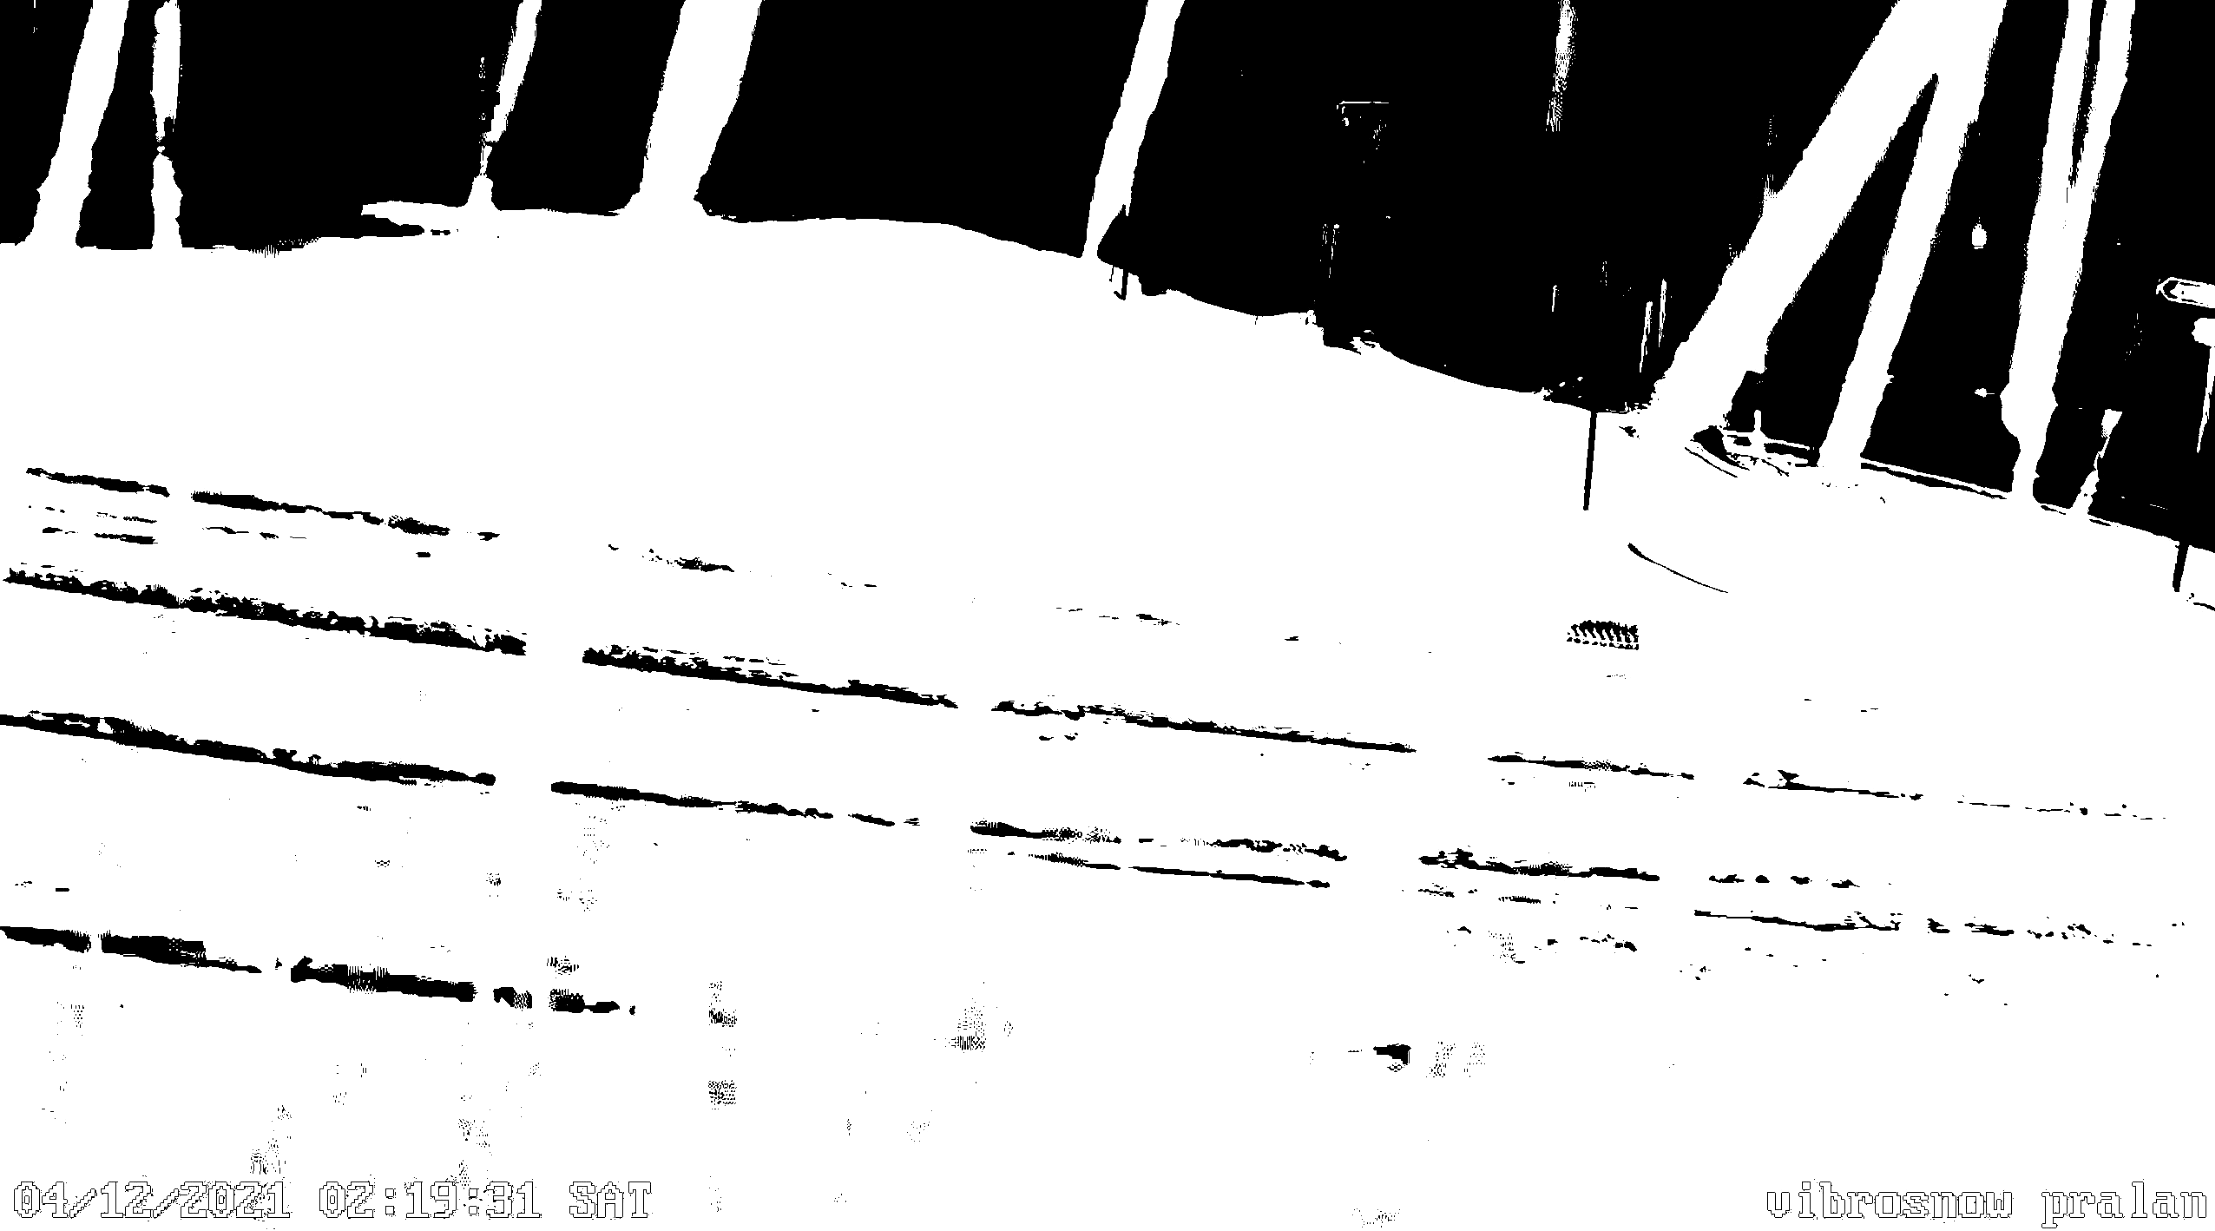
\includegraphics[width=\linewidth]{Images/computer_vision/snowOnRoad/test_thres.png}
        \caption{Image de test seuillée}
        \label{fig:SnowOnRoad_test_thres}
    \end{subfigure}
    \hfill
    \begin{subfigure}{.45\textwidth}
        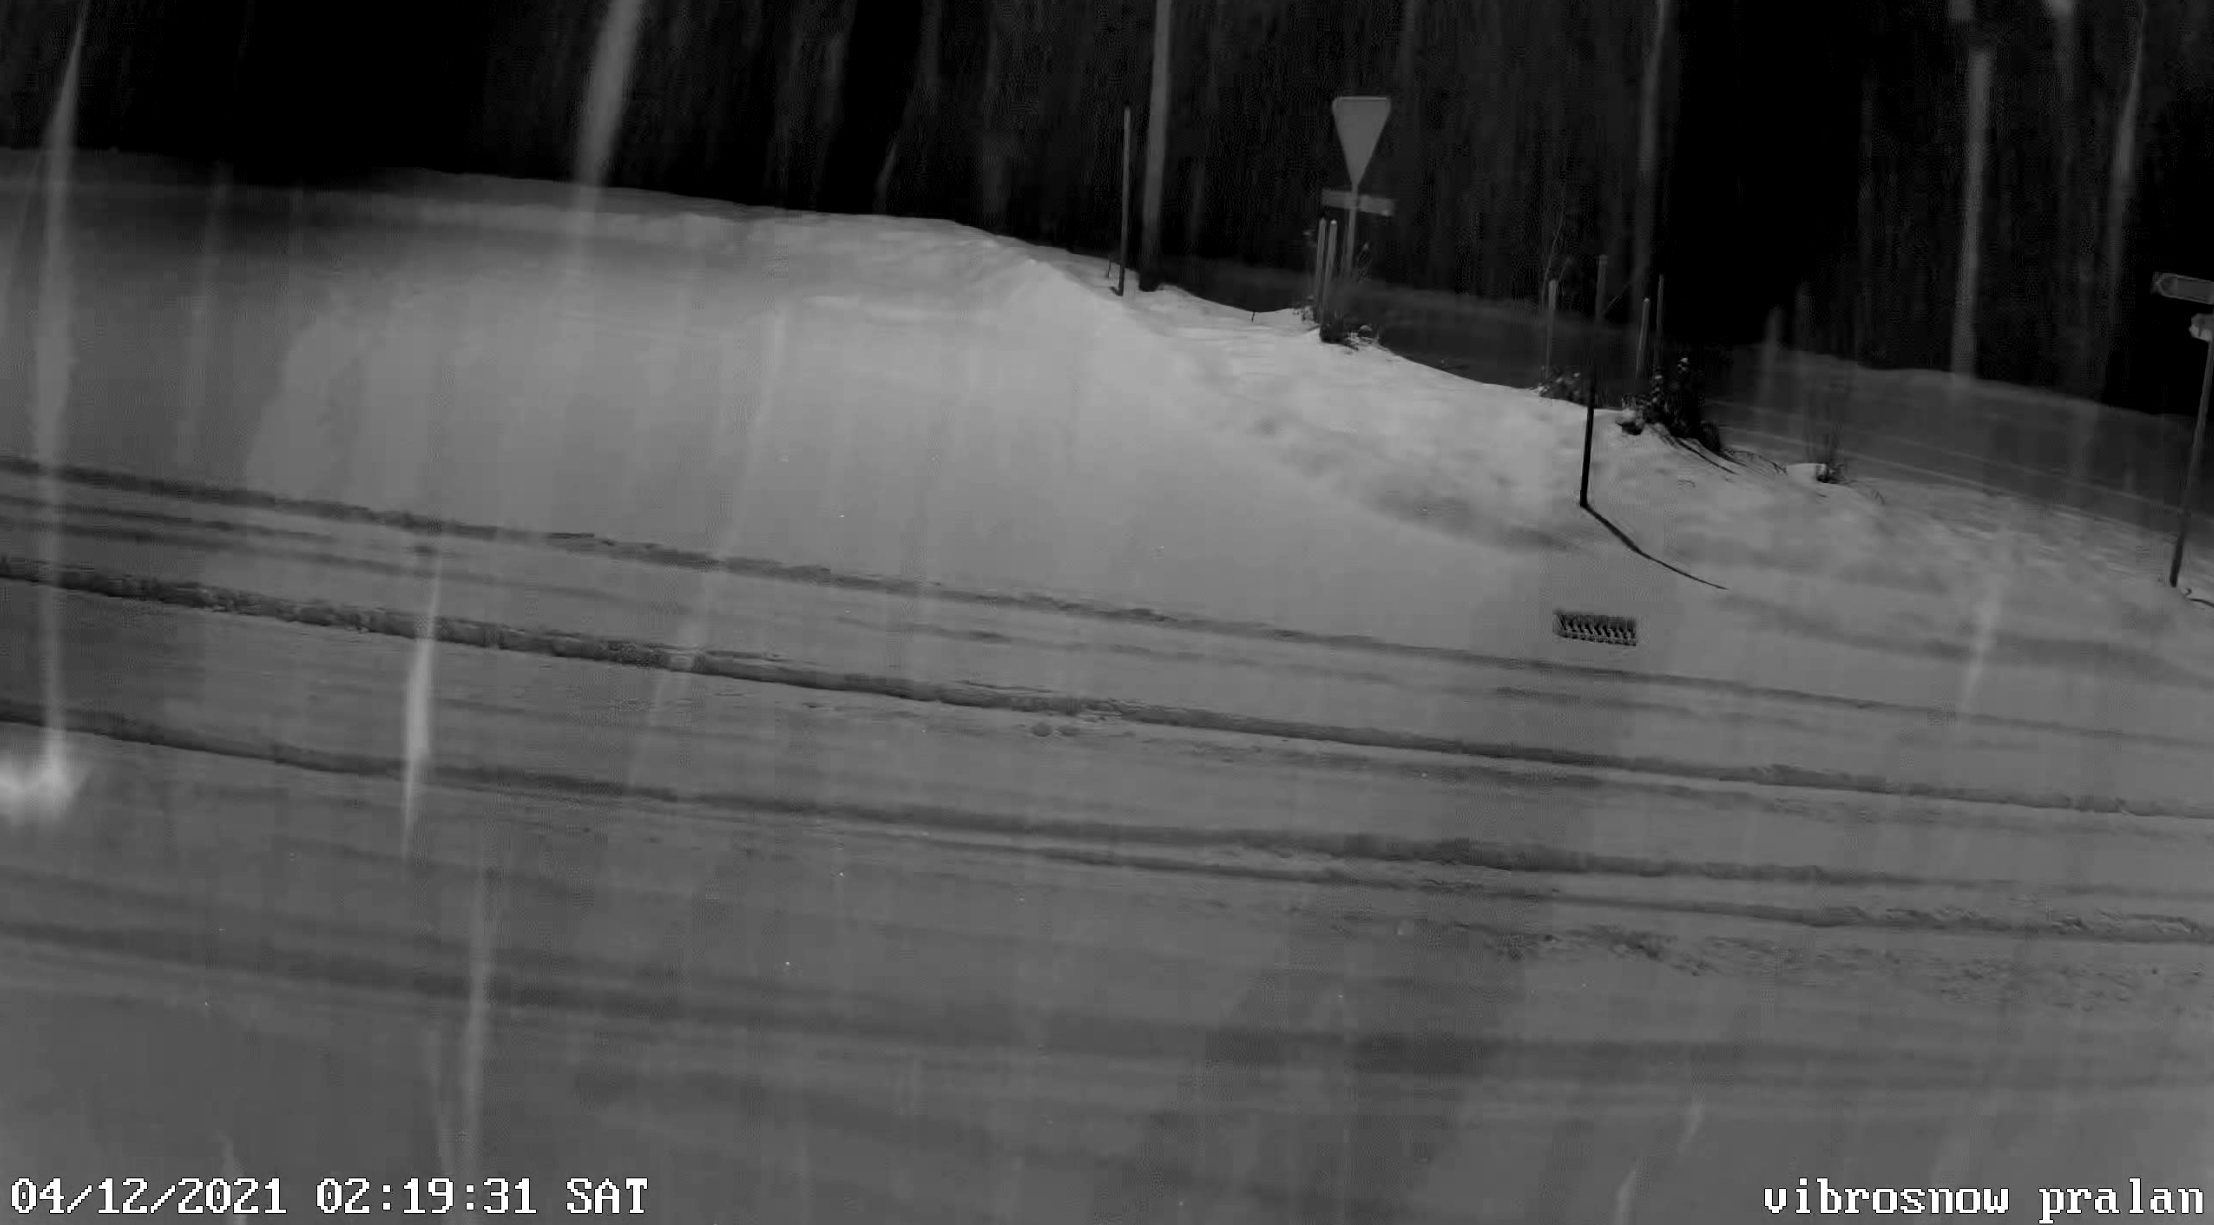
\includegraphics[width=\linewidth]{Images/computer_vision/snowOnRoad/test_denoised.png}
        \caption{Image de test avec suppression de bruit}
        \label{fig:SnowOnRoad_test_denoised}
    \end{subfigure}
    \hfill
    \begin{subfigure}{.45\textwidth}
        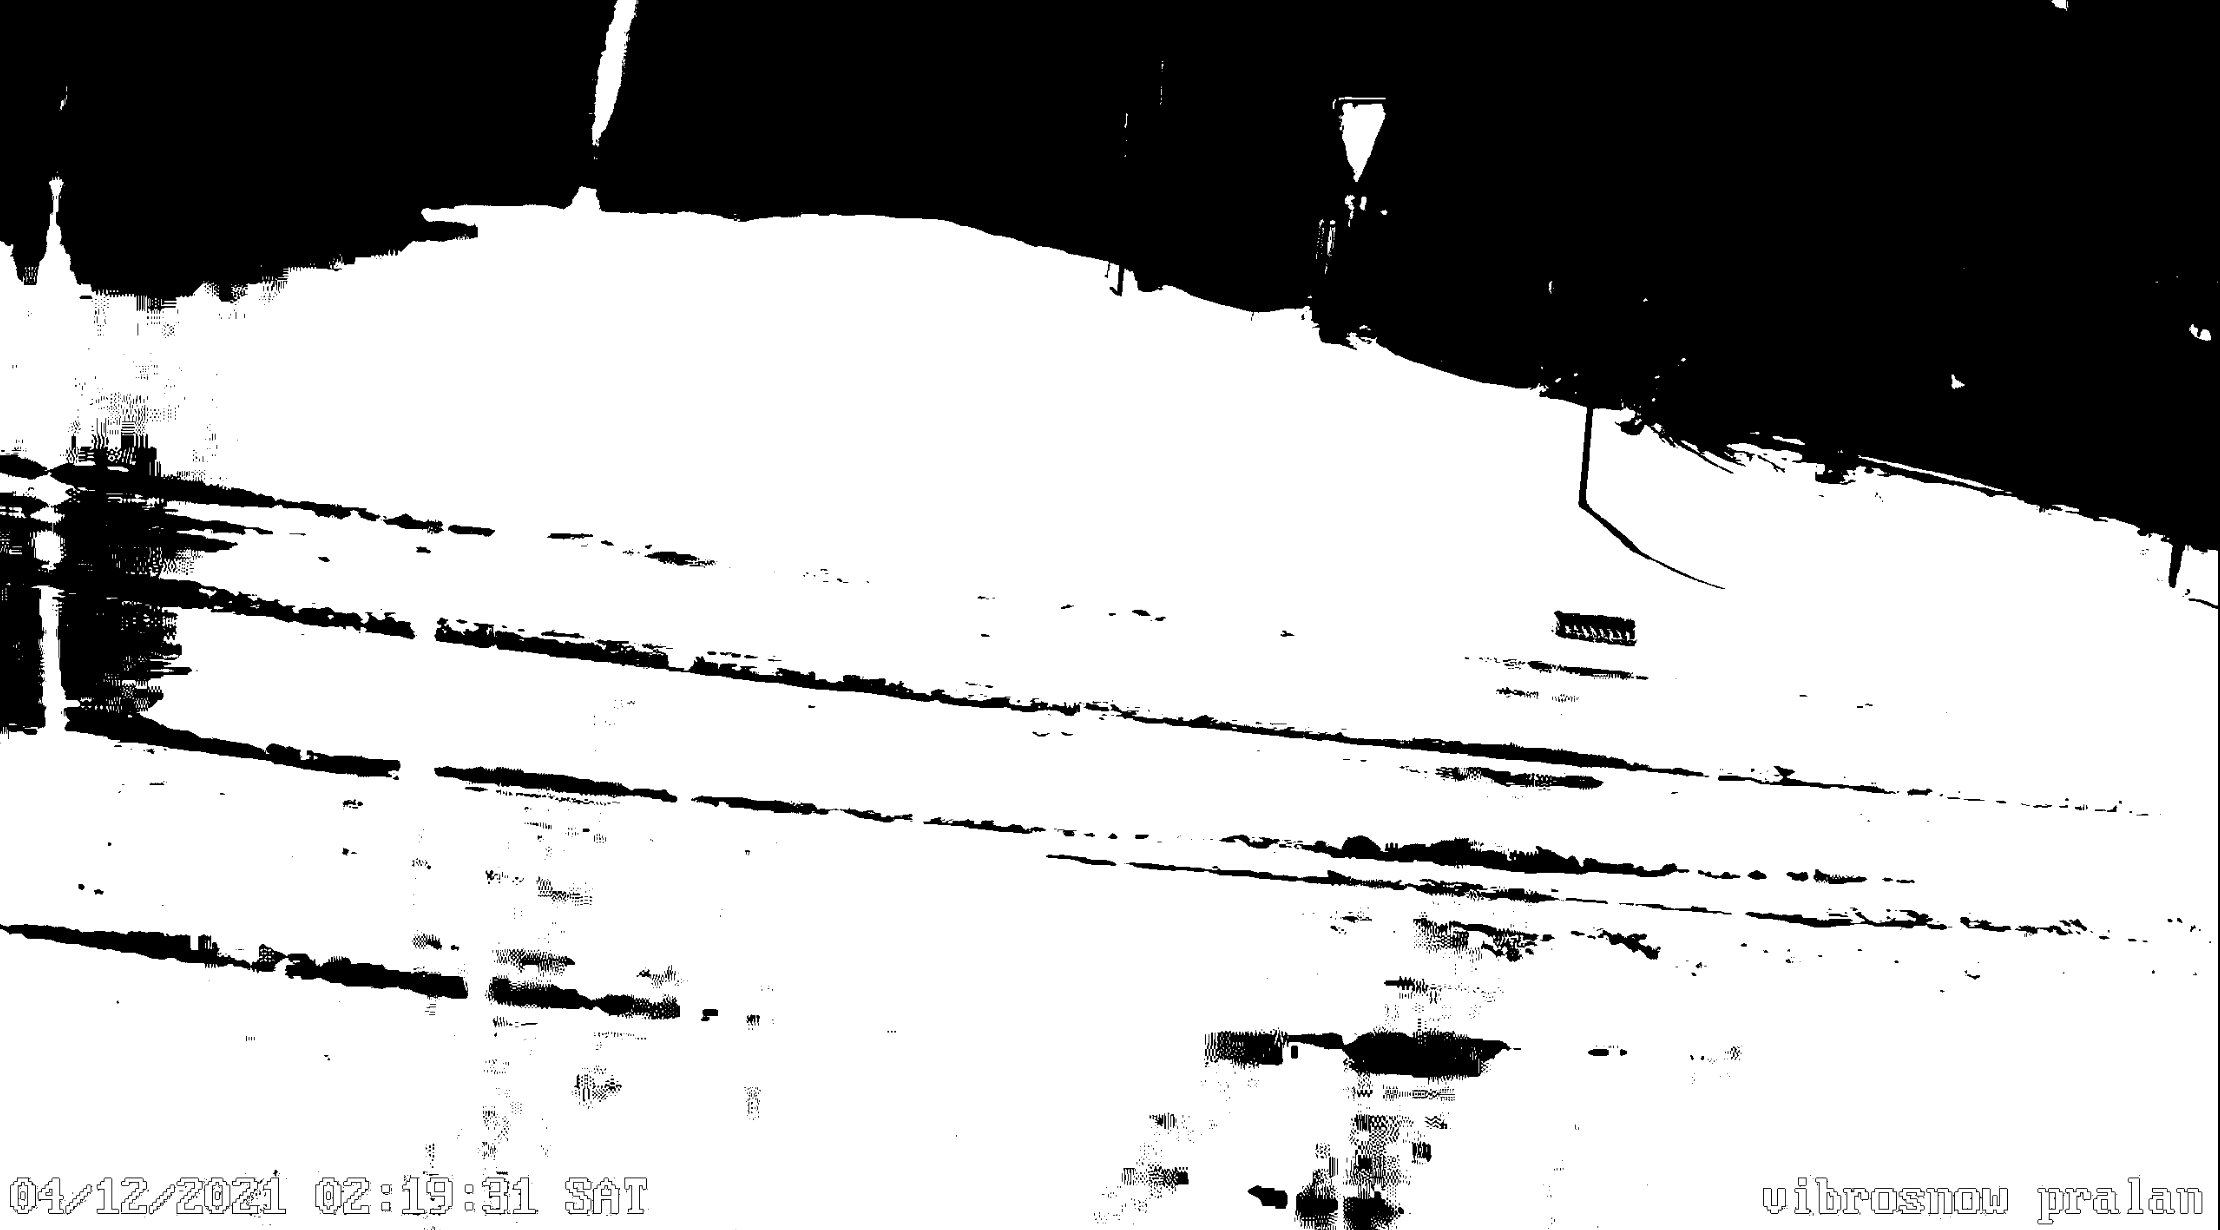
\includegraphics[width=\linewidth]{Images/computer_vision/snowOnRoad/test_denoisedThres.png}
        \caption{Image de test avec suppression de bruit et seuillée}
        \label{fig:SnowOnRoad_test_denoisedThres}
    \end{subfigure}
    \caption[Images testées pour détection de neige sur route]{Image de test}
    \label{fig:SnowOnRoad_test}
\end{figure}
\newpage